\documentclass{beamer}
\usepackage[utf8]{inputenc}
\usepackage[export]{adjustbox}
\usepackage{algorithmic}
\usepackage{amsmath}
\usepackage{commath}
\usepackage{dsfont}
\usepackage{graphicx}
\usepackage{hyperref}

\usepackage{amsfonts}
\usepackage{bm}

\newcommand{\bba}{{\mathbb A}}
\newcommand{\bbb}{{\mathbb B}}
\newcommand{\bbc}{{\mathbb C}}
\newcommand{\bbd}{{\mathbb D}}
\newcommand{\bbe}{{\mathbb E}}
\newcommand{\bbf}{{\mathbb F}}
\newcommand{\bbg}{{\mathbb G}}
\newcommand{\bbh}{{\mathbb H}}
\newcommand{\bbi}{{\mathbb I}}
\newcommand{\bbj}{{\mathbb J}}
\newcommand{\bbk}{{\mathbb K}}
\newcommand{\bbl}{{\mathbb L}}
\newcommand{\bbm}{{\mathbb M}}
\newcommand{\bbn}{{\mathbb N}}
\newcommand{\bbo}{{\mathbb O}}
\newcommand{\bbp}{{\mathbb P}}
\newcommand{\bbq}{{\mathbb Q}}
\newcommand{\bbr}{{\mathbb R}}
\newcommand{\bbs}{{\mathbb S}}
\newcommand{\bbt}{{\mathbb T}}
\newcommand{\bbu}{{\mathbb U}}
\newcommand{\bbv}{{\mathbb V}}
\newcommand{\bbw}{{\mathbb W}}
\newcommand{\bbx}{{\mathbb X}}
\newcommand{\bby}{{\mathbb Y}}
\newcommand{\bbz}{{\mathbb Z}}

\newcommand{\bma}{{\bm a}}
\newcommand{\bmb}{{\bm b}}
\newcommand{\bmc}{{\bm c}}
\newcommand{\bmd}{{\bm d}}
\newcommand{\bme}{{\bm e}}
\newcommand{\bmf}{{\bm f}}
\newcommand{\bmg}{{\bm g}}
\newcommand{\bmh}{{\bm h}}
\newcommand{\bmi}{{\bm i}}
\newcommand{\bmj}{{\bm j}}
\newcommand{\bmk}{{\bm k}}
\newcommand{\bml}{{\bm l}}
\newcommand{\bmm}{{\bm m}}
\newcommand{\bmn}{{\bm n}}
\newcommand{\bmo}{{\bm o}}
\newcommand{\bmp}{{\bm p}}
\newcommand{\bmq}{{\bm q}}
\newcommand{\bmr}{{\bm r}}
\newcommand{\bms}{{\bm s}}
\newcommand{\bmt}{{\bm t}}
\newcommand{\bmu}{{\bm u}}
\newcommand{\bmv}{{\bm v}}
\newcommand{\bmw}{{\bm w}}
\newcommand{\bmx}{{\bm x}}
\newcommand{\bmy}{{\bm y}}
\newcommand{\bmz}{{\bm z}}

\newcommand{\bmxi}{{\bm \xi}}

\newcommand{\bmA}{{\bm A}}
\newcommand{\bmB}{{\bm b}}
\newcommand{\bmC}{{\bm c}}
\newcommand{\bmD}{{\bm d}}
\newcommand{\bmE}{{\bm e}}
\newcommand{\bmF}{{\bm f}}
\newcommand{\bmG}{{\bm g}}
\newcommand{\bmH}{{\bm h}}
\newcommand{\bmI}{{\bm i}}
\newcommand{\bmJ}{{\bm j}}
\newcommand{\bmK}{{\bm k}}
\newcommand{\bmL}{{\bm l}}
\newcommand{\bmM}{{\bm m}}
\newcommand{\bmN}{{\bm n}}
\newcommand{\bmO}{{\bm o}}
\newcommand{\bmP}{{\bm p}}
\newcommand{\bmQ}{{\bm q}}
\newcommand{\bmR}{{\bm r}}
\newcommand{\bmS}{{\bm s}}
\newcommand{\bmT}{{\bm t}}
\newcommand{\bmU}{{\bm u}}
\newcommand{\bmV}{{\bm v}}
\newcommand{\bmW}{{\bm w}}
\newcommand{\bmX}{{\bm x}}
\newcommand{\bmY}{{\bm y}}
\newcommand{\bmZ}{{\bm z}}

\newcommand{\cala}{{\mathcal A}}
\newcommand{\calb}{{\mathcal B}}
\newcommand{\calc}{{\mathcal C}}
\newcommand{\cald}{{\mathcal D}}
\newcommand{\cale}{{\mathcal E}}
\newcommand{\calf}{{\mathcal F}}
\newcommand{\calg}{{\mathcal G}}
\newcommand{\calh}{{\mathcal H}}
\newcommand{\cali}{{\mathcal I}}
\newcommand{\calj}{{\mathcal J}}
\newcommand{\calk}{{\mathcal K}}
\newcommand{\call}{{\mathcal L}}
\newcommand{\calm}{{\mathcal M}}
\newcommand{\caln}{{\mathcal N}}
\newcommand{\calo}{{\mathcal O}}
\newcommand{\calp}{{\mathcal P}}
\newcommand{\calq}{{\mathcal Q}}
\newcommand{\calr}{{\mathcal R}}
\newcommand{\cals}{{\mathcal S}}
\newcommand{\calt}{{\mathcal T}}
\newcommand{\calu}{{\mathcal U}}
\newcommand{\calv}{{\mathcal V}}
\newcommand{\calw}{{\mathcal W}}
\newcommand{\calx}{{\mathcal X}}
\newcommand{\caly}{{\mathcal Y}}
\newcommand{\calz}{{\mathcal Z}}

\DeclareMathOperator*{\argmin}{arg\,min}
\DeclareMathOperator{\ind}{{\mathds 1}}

\usetheme{Warsaw}
\usefonttheme{professionalfonts}
% \usepackage{fontspec}
% \setmainfont{Times New Roman}

\title{Neural Networks}
\author{
    Yu Gai \\
    Instructed by Professor G\'erard Ben Arous
}

\begin{document}

\frame{\titlepage}

\begin{frame}

\frametitle{The probably approximately correct (PAC) learning framework}

\begin{itemize}
\item An input space $\calx \subset \bbr^d$
\item An output space $\caly$, either $\{\pm 1\}$ or $\bbr$
\item A probability measure $\bbp$ over $\calx$
\item An unknown mapping $y: \calx \mapsto \caly$
\item An i.i.d. sample $\{(\bmx_i, y_i)\}_{i = 1}^n$, where $\bmx_i \sim \bbp$ and $y_i = y(\bmx_i)$
\end{itemize}

\end{frame}

\begin{frame}

\frametitle{Empirical risk minimization (ERM)}

Choose a hypothesis $h$ from a hypothesis space $\calh$ by computing
\[
h^* \triangleq \argmin_{h \in \calh} \frac1n \sum_{i = 1}^n \ind_{h(\bmx_i) \ne y_i}
\]
when $\caly = \{\pm 1\}$, or
\[
h^* \triangleq \argmin_{h \in \calh} \frac1n \sum_{i = 1}^n (h(\bmx_i) - y_i)^2
\]
when $\caly = \bbr$.

\end{frame}

\begin{frame}

\frametitle{The perceptron model}

Consider the case $\caly = \bbr$.
The hypothesis space of perceptrons is
\[
\calh \triangleq \{h_{\bmw, b} : \bmw \in \bbr^d, b \in \bbr\}
\]
where
\[
h_{\bmw, b} (\bmx)
\triangleq \bmw^T \bmx + b
= \sum_{i = 1}^d \bmw_i \bmx_i + b
\]
is a perceptron.
Choose $\bmw$ and $b$ by computing
\begin{align*}
\argmin_{\bmw, b} \ell (\bmw, b)
& = \argmin_{\bmw, b} \frac1n \sum_{i = 1}^n (h_{\bmw, b} (\bmx_i) - y_i)^2 \\
& = \argmin_{\bmw, b} \frac1n \sum_{i = 1}^n (\bmw^T \bmx_i + b - y_i)^2
\end{align*}

\end{frame}

\begin{frame}

\frametitle{Interpretation of perceptron as neuron}

\begin{figure}
\centering
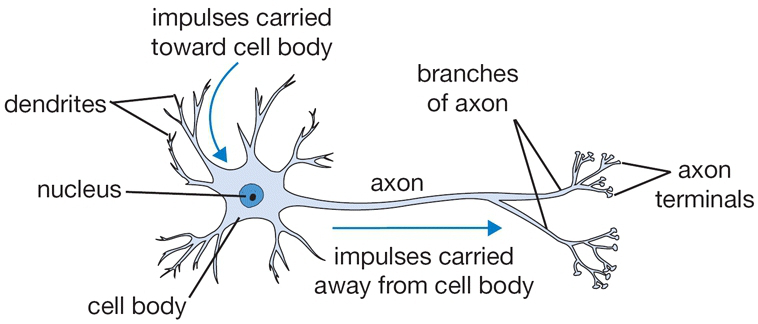
\includegraphics[scale=0.2, valign=t]{neuron}
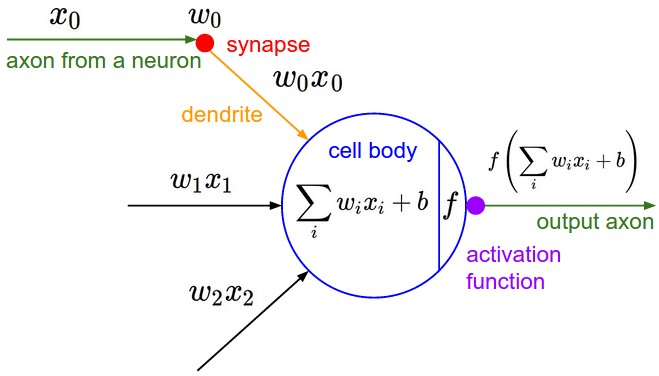
\includegraphics[scale=0.2, valign=t]{neuron_model}
\caption{Analogy between biological neuron and perceptron (figures from \url{http://cs231n.github.io/neural-networks-1/})}
\end{figure}

In the case of perceptron, the activation function is $\sigma (x) = x$.
Other choices of $\sigma$:
\[
\sigma (x) = \frac1{1 + \exp (-x)} \qquad
\sigma (x) = \tanh (x) \qquad
\sigma (x) = \max (0, x)
\]

\end{frame}

\begin{frame}

\frametitle{The limitation of perceptron: learning the \textsc{XOR} operation}

Consider the case $\calx = \caly = \{0, 1\}$, $\bbp$ is uniform over $\calx$, and
\[
y(\bmx)
= y(x_1, x_2)
= \textsc{XOR} (x_1, x_2) \triangleq \ind_{x_1 = x_2}
\]
\[
\{((0, 0), 1), ((1, 0), 0), ((0, 1), 0), ((1, 1), 1)\} \subset \{0, 1\}^2 \times \{0, 1\}
\]
$\bmw = (w_1, w_2) \subset \bbr^2$
\[
h_{\bmw, b} (\bmx) = w_1 x_1 + w_2 x_2 + b
\]
\[
\argmin_{w_1, w_2, b} \ell (\bmw, b) = ?
\]

\end{frame}

\begin{frame}

Solution: ``linear" combination of neurons with nonlinear activation function.

\[
g(\bmx) = \sum_{i = 1}^{d_1} v_i h_{\bmw_i, b_i} (\bmx) + a
\]
where
\[
h_{\bmw, b} (\bmx) = \sigma(\bmw^T \bmx + b)
\]
and $\bmw_i$ and $b_i$ are the weight and bias of the $i$th neuron.

Interpretation: a perceptron taking as input the activation of other neurons.

\begin{figure}
\centering
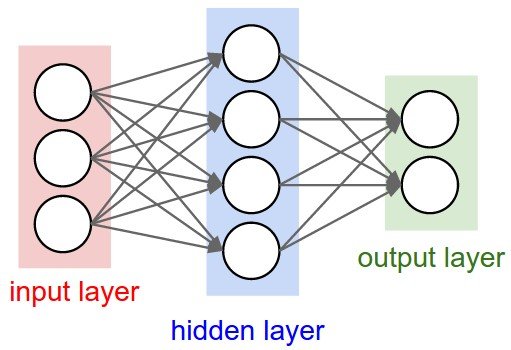
\includegraphics[scale=0.2, valign=t]{neural_net}
\caption{A neural network with one hidden layer (figure from \url{http://cs231n.github.io/neural-networks-1/})}
\end{figure}

\end{frame}

\begin{frame}

\frametitle{Vectorization}

More compactly,
\[
g(\bmx)
= \sum_{i = 1}^{d_1} v_i h_{\bmw_i, b_i} (\bmx) + a
= \bmv^T \sigma (W \bmx + \bmb) + a
\]
where $\bmv = [v_1, ..., v_{d_1}]$, the $i$th row of $W \in \bbr^{d_1 \times d}$ is $\bmw_i$, and $\bmb = [b_1, ..., b_{d_1}]^T$.
For $\bmv \in \bbr^d$ and $\sigma: \bbr \mapsto \bbr$,
\[
\sigma (\bmv) \triangleq [\sigma (v_1), ..., \sigma (v_d)]^T
\]
$\sigma (W \bmx + \bmb)$ is the activation of the hidden layer because $\sigma (W \bmx + \bmb)_i$ is the activation of the $i$th neuron.

\end{frame}

\begin{frame}

\frametitle{High-dimensional output}

Replace $\bmv \in \bbr^{d_1}$ by $V \in \bbr^{d_1 \times d_2}$ and $a \in \bbr$ by $\bma \in \bbr^{d_2}$ if $\caly \subset \bbr^{d_2}$:
\[
g(\bmx) = V \sigma (W \bmx + \bmb) + \bma
\]
Interpretation: multiple perceptrons taking as input the activation of a collection of neurons (the $i$th row of $V$ and $a_i$ are the weight and bias of the $i$th perceptron).

\end{frame}

\begin{frame}

\frametitle{Multi-layer perceptron (MLP)}

Replace input layer by hidden layer, i.e. $\bmx$ by $\sigma (W \bmx + \bmb)$, again, again, and again \ldots
\begin{align*}
\bmh_0 & = \bmx \\
\bmh_i & = \sigma (W_i \bmh_{i - 1} + \bmb_i) \qquad i = 1, ..., L - 1 \\
g(\bmx) & = W_L \bmh_{L - 1} + \bmb_L
\end{align*}
where $h_i$ is the activation of the $i$th hidden layer.

\begin{figure}
\centering
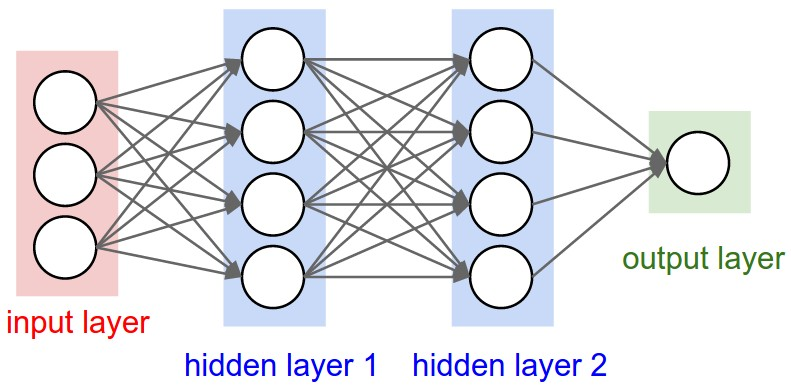
\includegraphics[scale=0.2, valign=t]{neural_net2}
\caption{An MLP with two hidden layers (figure from \url{http://cs231n.github.io/neural-networks-1/})}
\end{figure}

\end{frame}

\begin{frame}

\frametitle{The universal approximator theorem}

Let $\calh_{NN} \triangleq \{\text{neural network with one hidden layer}\}$.
$\calh_{NN}$ is a hypothesis space much richer than the space of perceptrons:
\begin{theorem}[\cite{cybenko1989approximation}]
$\calh_{NN}$ is dense in $C ([0, 1]^d)$.
\end{theorem}

There is no free lunch!
PAC-learnability lost:
\begin{corollary}
\[
d_{VC} \left(\left\{\ind_{h(\cdot) > \frac12} : h \in \calh_{NN}\right\}\right) = \infty
\]
\end{corollary}
Essentially a consequence of the universal approximator theorem and the fact that $C ([0, 1]^d)$ shatters any finite subset of $[0, 1]^d$.

\end{frame}

\begin{frame}

\frametitle{VC-dimension and PAC-learnability}

\begin{definition}
The \emph{VC-dimension} of a hypothesis space $\calh$ is defined as
\[
d_{VC} (\calh) \triangleq \max \{n : \Pi_\calh (n) = 2^n\}
\]
where for $n \in \bbn$,
\[
\Pi_\calh (n) \triangleq \max_{\{x_i\}_{i = 1}^n \subset \calx} |\{h(x_i)\}_{i = 1}^n : h \in \calh\}|
\]
\end{definition}

$\calh$ shatters $\{x_i\}_{i = 1}^n$ if $|\{h(x_i)\}_{i = 1}^n : h \in \calh\}| = 2^n$.
The VC-dimension of $\calh$ is the greatest $n$ such that $\calh$ shatters some subset of size $n$.

\begin{theorem}
\[
d_{VC} (\calh) < \infty
\Leftrightarrow \calh\ \text{is PAC-learnable (by ERM)}
\]
\end{theorem}

\end{frame}

\begin{frame}

\frametitle{Sketched proof of infinite VC-dimension}

It suffices to prove that $\left\{\ind_{h(\cdot) > \frac12} : h \in \calh_{NN}\right\}$ shatters any finite subset of $[0, 1]^d$.
$\forall n \in \bbn$, $\forall E \triangleq \{x_i\}_{i = 1}^n \subset [0, 1]^d$, $\forall F \subset E$, $\exists f \in C([0, 1]^d)$ s.t.
\[
f(F) = \{1\} \qquad f(E - F) = \{0\}
\]
Because $\calh_{NN}$ is dense in $C([0, 1]^d)$, $\forall \epsilon > 0$, $\exists h \in \calh_{NN}$ s.t.
\[
\sup_{\bmx \in [0, 1]^d} |f(\bmx) - h(\bmx)| < \epsilon
\]
In particular, $\exists h \in \calh_{NN}$ s.t.
\[
\max_{\bmx \in E} |f(\bmx) - h(\bmx)| < \frac14
\]

\end{frame}

\begin{frame}

\frametitle{Solution to lost PAC-learnability: structural risk minimization (SRM) \cite{vapnik1992principles}}

Motivation:
\begin{theorem}
Suppose $d_{VC} (\calh) < \infty$.
Then with probability at least $1 - \eta$,
\[
\forall h \in \calh, R (h) < \hat{R} (h) + \delta_\calh
\]
where
\[
\delta_\calh \triangleq \sqrt{\frac{d_{VC} (\calh) \left(\log \frac{2 n}{d_{VC} (\calh)} + 1\right) - \log \eta}{n}}
\]
\end{theorem}

\end{frame}

\begin{frame}

\frametitle{Structural risk minimization (continued)}

Suppose $\exists \calh_1 \subset \calh_2 \subset ...$ such that
\[
\calh = \bigcup_i^\infty \calh_i
\]
Let $h_i^* \triangleq \argmin_{h \in \calh_i} \hat{R} (h)$.
It follows that
\[
\hat{R} (h_1^*) \leq \hat{R} (h_2^*) \leq \ldots \qquad
\]
Also,
\[
d_{VC} (\calh_1) \leq d_{VC} (\calh_2) \leq \ldots
\Rightarrow \delta_{\calh_1} \geq \delta_{\calh_2} \geq \ldots
\]

Hopefully the upper bound $\hat{R}(h_i^*) + \delta_{\calh_i}$ is a U-shaped function of $i$ (analoguous to bias-variance trade-off).

\end{frame}

\begin{frame}

\frametitle{Structural risk minimization (continued)}

How to optimize a U-shaped function of one integer variable?

Let $U(i) \triangleq \hat{R}(h_i^*) + \delta_{h_i}$.
\begin{algorithmic}
\STATE $i \gets 1$
\WHILE{$U(i) \leq U(i + 1)$}
    \STATE $i \gets i + 1$
\ENDWHILE
\RETURN $i$
\end{algorithmic}

Algorithmically, SRM is feasible as long as ERM is feasible, i.e. it is feasible to compute $h_i^*$.

\end{frame}

\begin{frame}

\frametitle{SRM applied to $\calh_{NN}$}

Let $\calh_{NN}^n \triangleq \{\text{neural network with one hidden layer of size}\ n\}$.
\[
\calh_{NN} = \bigcup_{n = 1}^\infty \calh_{NN}^n
\]

Each $\calh_{NN}^n$ is a more restricted hypothesis space:
\begin{theorem}[\cite{maass1995vapnik}]
If $\sigma (x) = 1 / (1 + \exp (-x))$, then
\[
d_{VC} (\calh_{NN}^n) = \calo (m^4)
\]
where $m$ is the number of weights.
\end{theorem}

Consequence: neural networks with a fixed architecture is PAC-learable, and are not universal function approximators.
Gradient descent.

\end{frame}

\begin{frame}

\frametitle{SRM applied to $\calh_{NN}$ (continued)}

Apply SRM to the hypothesis familiy
\[
\calh_{NN}^1, \calh_{NN}^2, \ldots
\]
(although it is not the case that $\calh_{NN}^1 \subset \calh_{NN}^2 \subset \ldots$, why?)

It remains to compute
\[
h_i^* \triangleq \argmin_{h \in \calh_i} \hat{R} (h)
\]

\end{frame}

\begin{frame}

\frametitle{ERM with gradient descent}

As illustrated in class, fix $\calh_{NN}^i$ we can optimize
\[
\frac1n \sum_{i = 1}^n \ell(g(\bmx_i), y_i)
\]
with gradient descent for ``nice" surrogate loss functions $\ell$, although the optimization problem now is always non-convex.

However, you can still give it a try!

We can use the chain rule to compute gradient (a.k.a. backward propagation).
Hopefully you have mastered the chain rule by now. If not \ldots

\end{frame}

\begin{frame}

\frametitle{Limitation of SRM}

Approximation complexity:
``[B]esides a negligible set, all functions that can be implemented by a deep network of polynomial size, require exponential size in order to be realized (or even approximated) by a shallow network."\cite{cohen2016expressive}

Consider neurons $\{f_{\bmw, b}\}$ a basis indexed by $\bmw \in \bbr^d$ and $b \in \bbr$.
A complete basis can have high approximation complexity for some functions.

Forget about \emph{universal} approximators and instead look for ``good" (in the language of mathematicians) bases/(in the language of alchemists) architectures!

What does ``good" mean?

\end{frame}

\begin{frame}

\frametitle{Convolutional neural networks (CNN) for image classification}

An image is a mapping $f: \bbr^2 \rightarrow \bbr^C$ with compact support, where $C$ is the number of channels ($C = 1$ for grayscale image, $C = 3$ for RBG image).

Assume the support is $[0, 1]^2$.

After discretizing $[0, 1]^2$: $\bmx \in \bbr^{W H C}$.

\end{frame}

\begin{frame}

\frametitle{Fourier transform essentials}

\begin{definition}
The Fourier transform $\calf f$ of $f \in L^1 (\bbr^d)$ is defined as
\[
(\calf f) (\bmxi) \triangleq \int_{\bbr^d} e^{-i \bmxi^T \bmx} f(\bmx) \dif \bmx
\]
The inverse Fourier transform $\calf f$ of $f \in L^1 (\bbr^d)$ is defined as
\[
(\calf f) (\bmx) \triangleq \int_{\bbr^d} e^{i \bmx^T \bmxi} f(\bmxi) \dif \bmxi
\]
\end{definition}

\end{frame}

\begin{frame}

\frametitle{Fourier transform essentials (continued)}

$L^2 (\bbr^d)$ is a Hilbert space when equipped with the inner product
\[
\langle f, g\rangle_{L^2 (\bbr^d)} \triangleq \int_{\bbr^d} f \bar{g} \dif \mu \qquad \forall f, g \in L^2 (\bbr^d)
\]
where $\mu$ denotes the Lebesgue measure of $\bbr^d$.

\begin{theorem}[Plancherel]
\langle f, g\rangle_{L^2 (\bbr^d)} = \frac1{(2 \pi)^d} \langle \calf f, \calf g\rangle_{L^2 (\bbr^d)} \qquad \forall f, g \in L^1 (\bbr^d) \cap L^2 (\bbr^d)
\end{theorem}

Fact: $L^1 (\bbr^d) \cap L^2 (\bbr^d)$ is dense in $L^2 (\bbr^d)$.

Consequence: $\calf f$ for $f \in L^2 (\bbr^d) - L^1 (\bbr^d)$ can be defined as the limit of
\[
\{\calf f_n\}_{n = 1}^\infty \subset L^1 (\bbr^d) \cap L^2 (\bbr^d)
\]
where $f_n \rightarrow f$ and all convergence is in norm.

\end{frame}

\begin{frame}

\frametitle{Convolution}

The convolution $k * f$ of $f \in L^1 (\bbr^d) \cap L^2 (\bbr^d)$ with $k \in L^1 (\bbr^d) \cap L^2 (\bbr^d)$ is defined as
\[
(k * f) (\bmy) \triangleq \int_{\bbr^d} k(\bmy - \bmx) f(\bmx) \dif \bmx
\]
where $f$ is interpreted as a signal (e.g. an image), and $k$ is interpreted as a kernel.

\begin{theorem}
\[
k * f = \calf^{-1} ((\calf k) \cdot (\calf f))
\]
\end{theorem}

Interpretation: filtering in the Fourier domain.

\end{frame}

\begin{frame}

\frametitle{Discretized convolution}

\begin{figure}
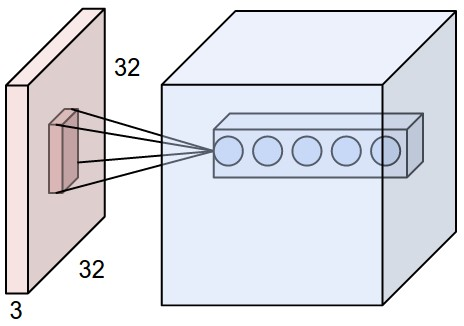
\includegraphics[scale=0.2]{depthcol}
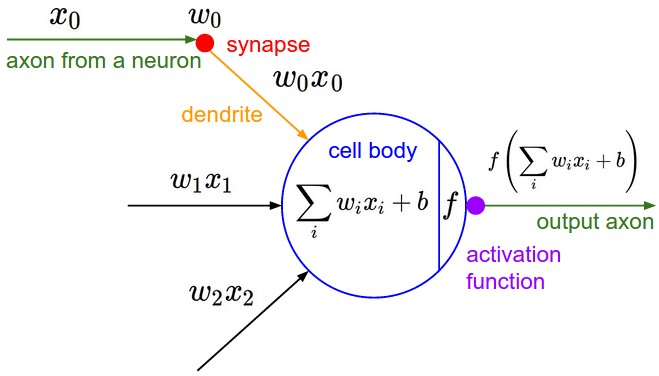
\includegraphics[scale=0.2]{neuron_model}
\caption{Convolution (figure from \url{http://cs231n.github.io/convolutional-networks/})}
\end{figure}
\end{frame}

\end{frame}

\begin{frame}

\frametitle{Downsampling tricks}

\begin{figure}
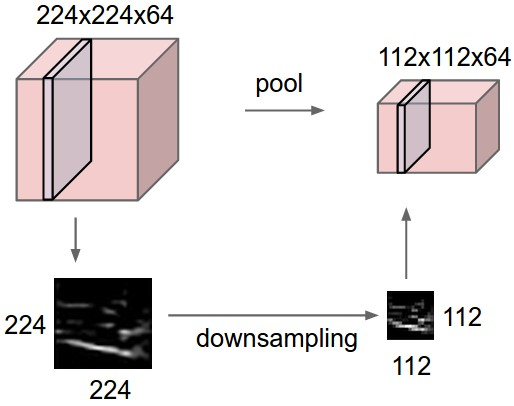
\includegraphics[scale=0.2]{pool}
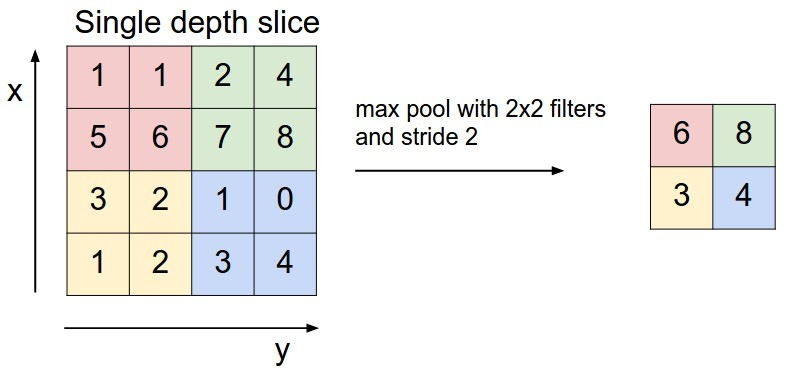
\includegraphics[scale=0.2]{maxpool}
\caption{Pooling (figure from \url{http://cs231n.github.io/convolutional-networks/})}
\end{figure}
\end{frame}

\begin{frame}

\frametitle{Example: LeNet}

\begin{figure}
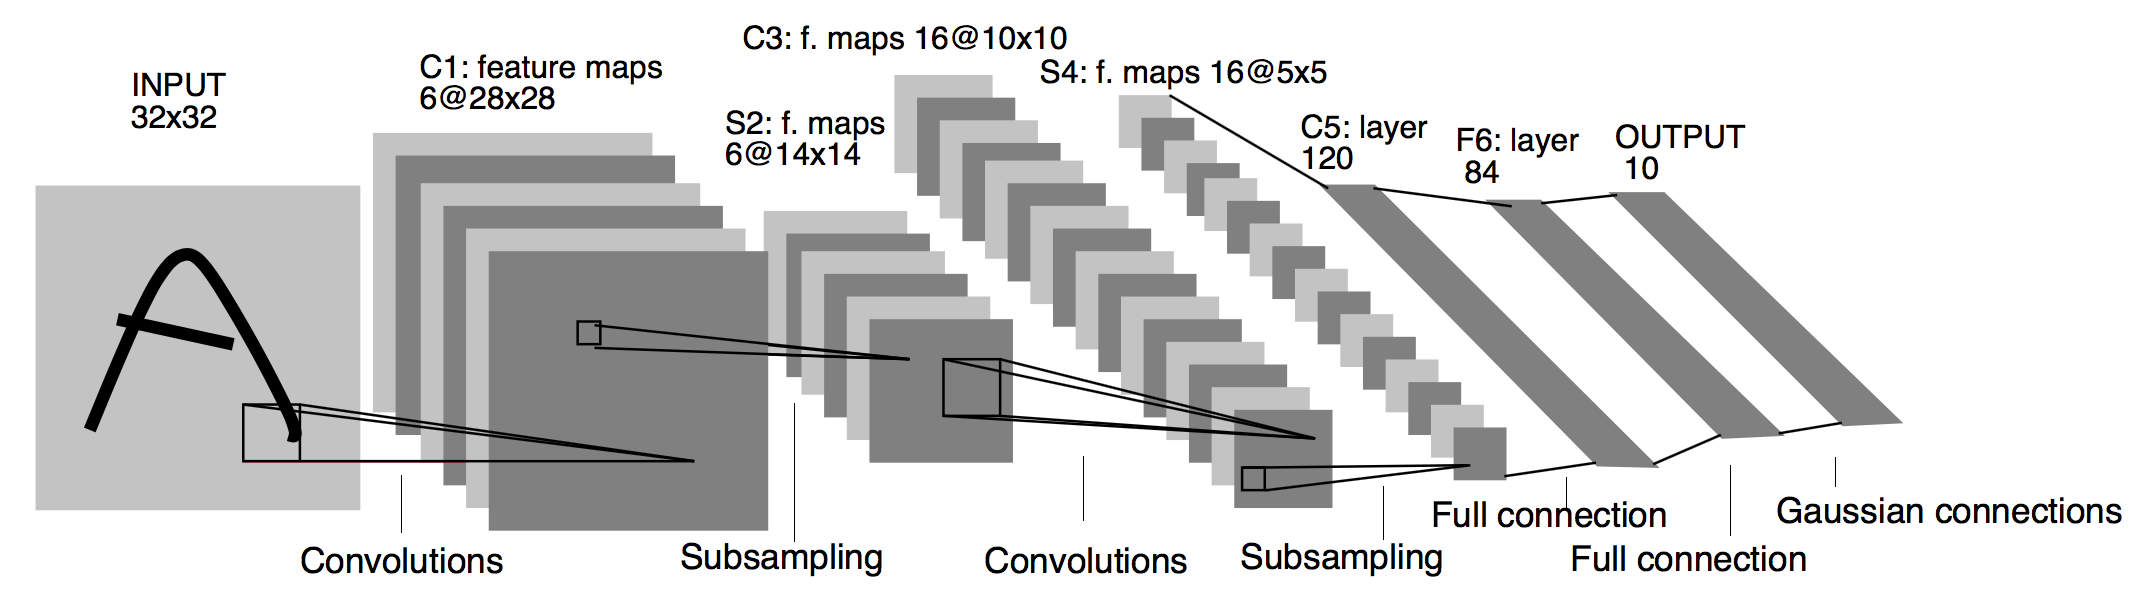
\includegraphics[scale=0.1]{lenet}
\caption{The architecture of LeNet (figure from \cite{lecun1998gradient})}
\end{figure}

\end{frame}

\begin{frame}

\frametitle{Invariance}

Displacement/Deformation field:
\[
\tau: \bbr^d \mapsto \bbr^d \in \calc^2
\]
Displacement/Deformation operator:
\[
(\call_\tau f) (\bmx) \triangleq f(\bmx - \tau (\bmx))
\]
Example (translation):
\[
\tau (\bmx) = \bmc \qquad
(\call_\tau f) (\bmx) = f(\bmx - \bmc)
\]

\end{frame}

\begin{frame}

\frametitle{Translation invariance}

Convolution is translation invariant because
\begin{align*}
(k * (\call_\tau f)) (\bmy)
& = \int_{\bbr^d} k(\bmx) (\call_\tau f) (\bmy - \bmx) \dif \bmx \\
& = \int_{\bbr^d} k(\bmx) f(\bmy - \bmx - \bmc) \dif \bmx \\
& = \int_{\bbr^d} k(\bmx) f((\bmy - \bmc) - \bmx) \dif \bmx \\
& = (k * f) (\bmy - \bmc) \\
& = (\call_\tau (k * f)) (\bmy)
\end{align*}

Why is MLP not translation invariant?

Open question: for what kind of kernels is convolution deformation-invariant?

\end{frame}

\begin{frame}

\frametitle{The belief in information bottleneck}

\cite{mallat2012group} shows how to construct a deformation-invariant kernel.

However, is it the best kernel?

Learning with information bottleneck may result in better kernels.

\end{frame}

\begin{frame}[allowframebreaks]

\bibliographystyle{unsrt}
\bibliography{presentation}

\end{frame}

\end{document}
